%% ------------------------------------------------------------------------- %%
\chapter{Introdução}
\label{cap:introducao}

O avanço e descoberta de novas tecnologias faz parte da história da humanidade. Em economia cunha-se o termo \textit{General Pupose Technology}, que são avanços tecnológicos que afetam toda uma economia. Entre estes avanços tecnológicos temos o motor a vapor, posteriormente substituído pelo motor a combustão interna. O computador representou um avanço tecnológico. A internet representou um grande salto na maneira como são feitas as comunicações e transações financeiras hoje. E atualmente, inteligência artificial está caminhando para romper esta barreira e impactar toda a economia \todo{adicionar referências}.

As primeiras redes neurais foram concebidas em 1945, o famoso perceptron. Mas desde 1945 e até os dias atuais, a área de inteligência artificial passou por vários momentos. Dentre eles momentos de euforia, no qual pesquisadores e entusiastas já previam rôbos substituindo o ser humano e que todas as tarefas seriam feitas pelos computadores. E momentos de pouco investimento, chamado \textit{AI Winter}, devido as muitas expectativas e poucos resultados. Porém demorou pelo menos 50 anos para termos os primeiros indícios do potencial desta área. Inteligência artificial abrange várias áreas. E a área que mais se destaca atualmente é a área de aprendizagem de máquina. Mais especificamente aprendizagem de máquina profunda. \todo{corrigir este parágrafo. Adicionar datas certas}

Alan Turing após conceber o primeiro computador em 1930 (ver data e se está correto), disse que o computador poderia resolver qualquer problema desde que fosse possível passar as regras. O computador resolve facilmente operações aritméticas e até mesmo consegue ganhar de um campeão mundial de xadrez (1997). Porém, tarefas que são simples para o ser humano como reconhecer faces, falas ou traduzir textos, são tarefas muito complexas para o computador, pois o ser humano não consegue traduzir estas ações em regras ou fórmulas para o computador. \todo{corrigir}

Porém, estes desafios de reconhecimento de imagens e tradução de textos foram superados pela máquina em 2015. Uma competição ImageNET no qual vários pesquisadores competem entre si para reconhecer milhares de imagem do banco imagenet. Um grupo do canadá apresentou o CNN, uma rede neural convolucional profunda no qual obteve 70\% de acurácia.

No ano posterior, ele obteve 97\%. Este desafio foi dado como superado. Não foi somente reconhecimento de imagens que o computador igualou e superou o ser humano. A IBM desenvolveu um computador que ganhou do ser humano no \textit{Jeopardy}. O Google desenvolveu o \textit{Alpha Go} que superou o campeão mundial de Go.

Todas estas conquistas feitas por pesquisadores e especialistas da área de inteligência artificial, foram feitas utilizando redes neurais profundas, mais especificamente redes neurais convolucionais e recorrentes. Tanto as redes convolucionais e redes recorrentes já eram conhecidas desde a década de 90. Com algumas exceções e outros detalhes, a maioria dos algoritmos já haviam sido desenvolvidas na década de 80 e 90. Porém só em 2015 o primeiro resultado veio a tona.

Neste período de 20 a 30 anos, ocorreram evoluções em outras áreas da computação que permitiu o salto em aprendizagem de máquina. Os principais fatores que contribuíram foram:

\begin{itemize}
    \item Aumento do processamento de CPU e GPU. Temos também pesquisas avançando em processadores específicos para a área de inteligência artificial como os TPUs
    \item Aumento da capacidade de armazenagem
    \item Acesso e democratização da internet, que permitiu gerar um grande volume de dados
\end{itemize}

Há outros fatores, mas estes fatores foram cruciais para o advento e o salto da aprendizagem de máquina atual. E atualmente cada vez mais empresas e governos estão investindo dinheiro na área de inteligência artificial. Há demandas para uso na área agrícola, investimentos, saúde, comércio. Empresas como o Google, IBM, Facebook, Apple e Amazon estão investindo bilhões de dólares nesta área. E uma das áreas que de aprendizagem de máquina é o processamento de linguagem natural. 

A área de processamento de linguagem natural pesquisa e trabalha com diversos problemas. Entre eles temos a tradução de textos, geração de textos \todo{verificar as areas de NLP} e um problema bastante comum é a solução de perguntas e respostas. O problema da pergunta e respostas consiste basicamente em dado uma pergunta e um conjunto de possíveis respostas, o algoritmo deve selecionar qual ou quais respostas respondem aquela pergunta.

Normalmente este problema consiste em perguntas e respostas de no máximo 1 parágrafo. É um desafio hoje criar modelos que dado uma pergunta, consiga responder com um artigo. Ou dado um livro ou artigo, responder perguntas a respeito \todo{adicionar referências}. Tanto que o próprio Google anunciou em janeiro de 2019, uma competição no qual deve-se criar um modelo capaz de responder ou não a perguntas, extraindo informação de artigos do Wikipedia. https://ai.googleblog.com/2019/01/natural-questions-new-corpus-and.html

A competição tem uma base aberta para os interessados. É possível conferir o ranking também dos modelos propostos pelos pesquisadores: https://ai.google.com/research/NaturalQuestions/leaderboard


A partir de uma base de conhecimento, FAQ, empresas e governos podem utilizar um modelo treinado neste contexto para responder perguntas e dúvidas de usuários. Ao fazer pesquisa no \textit{Google}, ele exibe perguntas e respostas sobre determinados tópicos pertinentes ao assunto buscado. Normalmente referem-se a dúvidas comuns de usuários. Exemplo está na figura \ref{fig:busca-google}.

\begin{figure}[h]
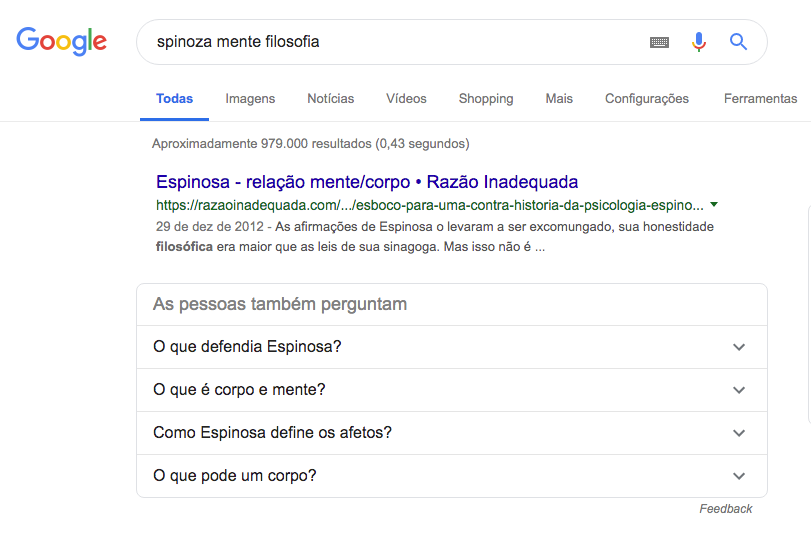
\includegraphics[width=12cm]{src/figuras/cap-introducao/busca-google-pergunta-resposta.png}
\caption{Perguntas relacionadas a pesquisa. Google and the Google logo are registered trademarks of Google LLC, used with permission.}
\label{fig:busca-google}
\end{figure}

Este problema de perguntas e respostas consiste em criar um modelo capaz de responder a dúvidas de usuários. A maioria das pesquisas atuais trabalham com linguagens naturais. Então, o usuário faz uma pergunta numa linguagem natural e o modelo responde com um texto em linguagem natural. Um outro desafio é dado uma pergunta em linguagem natural, estes modelos são capazes de responder em linguagem estruturada como XML, código fonte de linguagens como Java e/ou Python? 








%% ------------------------------------------------------------------------- %%
\section{Considerações Preliminares}
\label{sec:consideracoes_preliminares}


 Texto texto texto texto texto texto texto texto texto texto texto texto texto
texto texto texto texto texto texto texto texto texto texto texto texto texto
texto texto texto texto texto texto.

%% ------------------------------------------------------------------------- %%
\section{Objetivos}
\label{sec:objetivo}

Texto texto texto texto texto texto texto texto texto texto texto texto texto
texto texto texto texto texto texto texto texto texto texto texto texto texto
texto texto texto texto texto texto.

%% ------------------------------------------------------------------------- %%
\section{Contribuições}
\label{sec:contribucoes}

As principais contribuições deste trabalho são as seguintes:

\begin{itemize}
  \item Item 1. Texto texto texto texto texto texto texto texto texto texto
  texto texto texto texto texto texto texto texto texto texto.

  \item Item 2. Texto texto texto texto texto texto texto texto texto texto
  texto texto texto texto texto texto texto texto texto texto.

\end{itemize}

%% ------------------------------------------------------------------------- %%
\section{Organização do Trabalho}
\label{sec:organizacao_trabalho}

No Capítulo~\ref{cap:conceitos}, apresentamos os conceitos ... Finalmente, no
Capítulo~\ref{cap:conclusoes} discutimos algumas conclusões obtidas neste
trabalho. Analisamos as vantagens e desvantagens do método proposto ... 

As sequências testadas no trabalho estão disponíveis no Apêndice \ref{ape:sequencias}.
